\runningheader{Oppgave i)}{}{Side \thepage\ av \numpages}

\item[]   Alle modellene i denne delen av øvingen skal implementeres
  i subsystemet\\
  {\sf  Om Lookup Table-blokken, oppgave 2i)-2l)} i 
  skallfilen \fbox{\tt oving2.slx}.


  % ********************************************************
  % oppgave i) 
  % ********************************************************  
\item
  I denne oppgaven skal du begynne på en ny modell.
  Tettheten til vann som funksjon av temperatur er vist i figuren
  under
  \begin{figure}[H]
    \centering
    \scalebox{0.45}{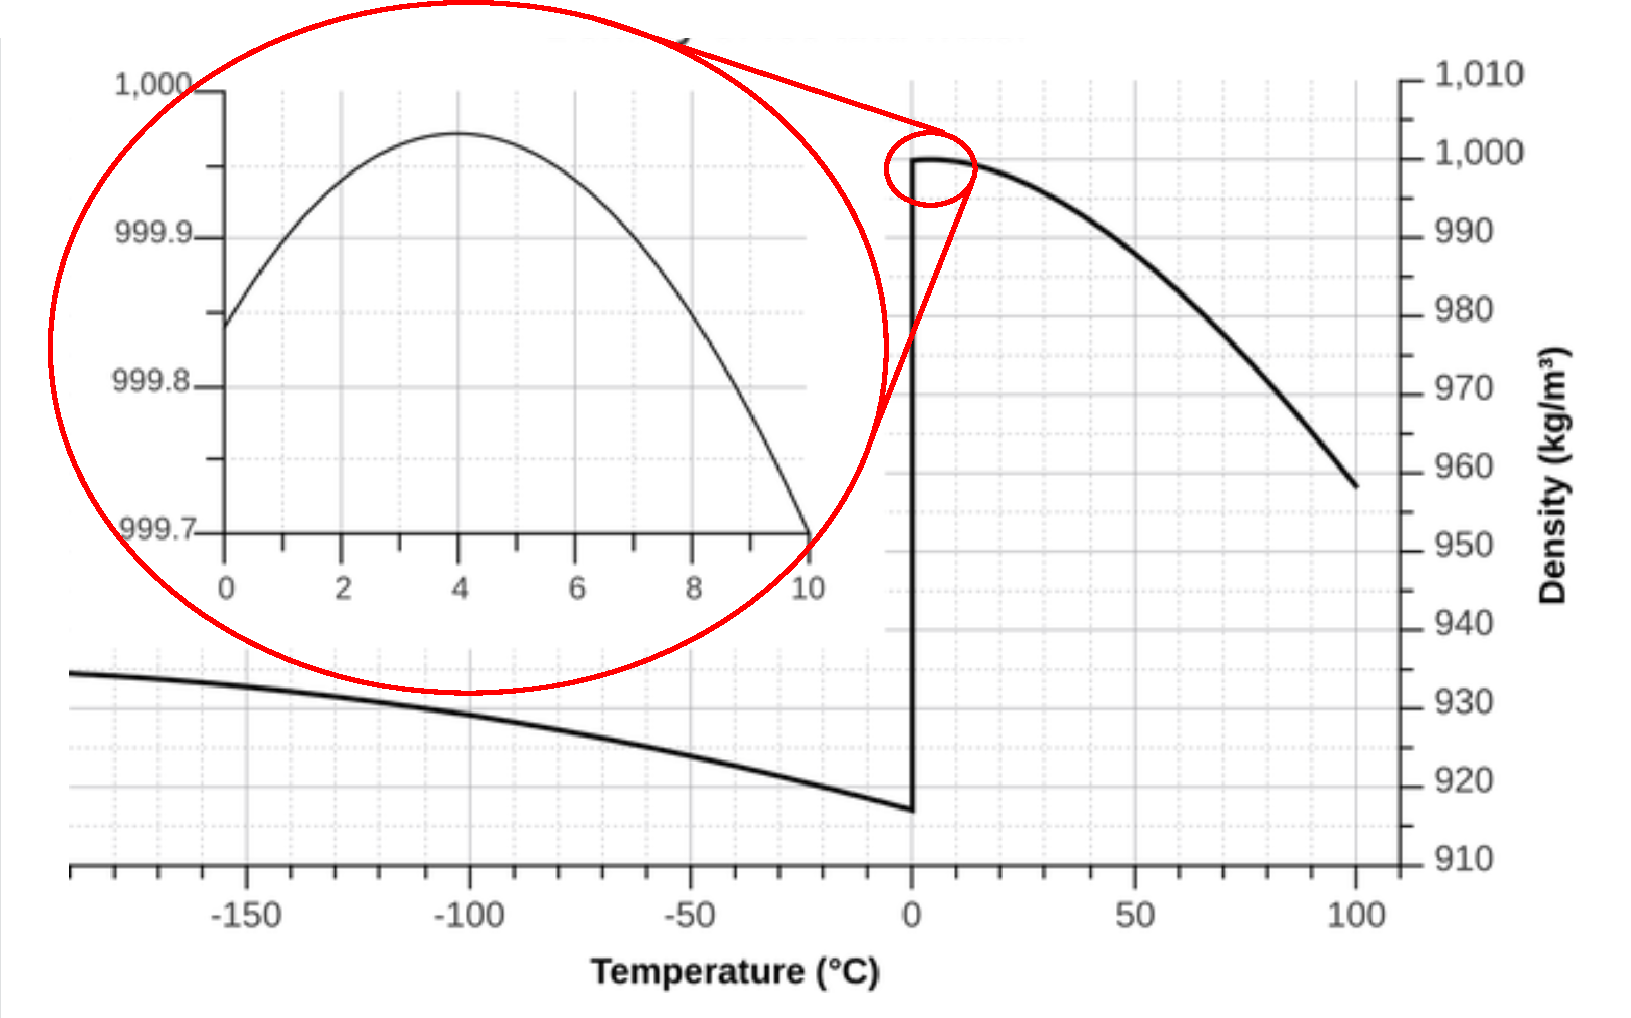
\includegraphics{tetthet_vann.pdf}} 
    \caption{Tettheten vann som funksjon av temperatur. Detaljene mellom
      0 og 10 grader er vist i egen delfigur.}   
    \label{fig:tetthet_vann}
  \end{figure}

  Målet med oppgaven er å implementere sammenhengen i
  figur~\ref{fig:tetthet_vann} i en {\sf  1-D Lookup table}-blokk
  som tar temperatur som et inngangssignal og gir ut tetthet som
  utgangssignal. Denne type blokk brukes for å implementere sammenhenger
  som ikke kan uttrykkes matematisk med en ligning.
  Blokken må spesifiseres med to vektorer med
  tallverdier som representerer kombinasjoner av verdier fra henholdsvis
  x-aksen og
  y-aksen. Ved å interpolere mellom punktene får du en kontinuerlig
  sammenhengen mellom inngangssignalet og 
  utgangssignalet.

  For å få med endringene i tetthet rundt $0^{\circ}$C
  samt detaljene mellom 0 og $10^{\circ}$C vist i  delfiguren i
  figur~\ref{fig:tetthet_vann}, så tar vi 
  utgangspunkt i følgende vektor med 
  temperaturer fra $-150^{\circ}$C til 
  $100^{\circ}$C. Om du vil kan du legge inn flere punkter selv. 

  {\tt T = [-150, -100, -50, -0.001, 0, 2, 4, 6, 8, 10, 30, 50, 70, 100]}

  \begin{itemize}
  \item Åpne skallfilen \fbox{\tt oving2\_data.m} og 
    fullfør den tilhørende vektoren \fbox{\tt rho} med tettheter avlest fra
    figur~\ref{fig:tetthet_vann}. Dette innebærer at for hver verdi i
    vektoren \fbox{\tt T} ovenfor, så leser du av tilhørende tetthet fra
    figuren.

    Ved å kjøre .m-filen får du en figur som viser sammenhengen slik at du
    får bekreftet at du har avlest riktige verdier og riktig antall
    verdier. Hensikten med å bruke en .m-fil først er at det er lettere å
    oppdage feil der enn i selve {\sf Lookup Table}-blokken.   


  \item I Simulinkmodellen henter du inn en {\sf 1-D Lookup table}-blokk
    hvor du benytter disse to
    vektorene til å spesifisere blokken. Du kan nå velge å enten
    kopiere inn vektorene med tallverdier i feltene
    eller skrive \fbox{\tt rho} og \fbox{\tt T} i feltene. Dette
    betinger at du kjører .m-filen først slik av disse variablene er
    tilgjengelig i {\sf Workspace}.

  \item     Måten {\sf 1-D Lookup table}-blokken interpolerer på er bestemt i fanen {\sf  Algorithm}
    under {\sf Interpolation method}. Defaultverdien er som du ser {\sf
      Linear point   slope}.

    
  \item   Fronten på blokken vil vise
    sammenhengen mellom temperatur og tetthet som vist under
    \begin{figure}[H]
      \centering
      \hspace*{0mm}\scalebox{0.8}{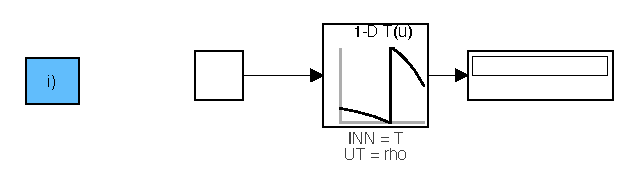
\includegraphics{2i.pdf}}
    \end{figure}

  \end{itemize}

    Inngangen kommer fra en {\sf  Constant}-blokk som representerer 
    temperaturen, og 
    utgangen går til 
    en {\sf  Display}-blokk som viser tilhørende
    tetthet. Du kan dobbelklikke på {\sf Display}-blokken og velge
    \dbox{\sf Numeric  display format} som {\sf Long}.   

    
  {\bf Gjør følgende oppgaver / svar på følgende spørsmål:    }
  
    \begin{enumerate}[label=i\arabic*)]
\item  Skriv inn en av temperaturene fra vektoren {\tt T} og sjekk at
    resultatet gir den verdien du har lest ut fra grafen. Hvilken
    temperatur valgte du, og hvilken tetthetsverdi fikk du ut?

  \item Benytt figur~\ref{fig:tetthet_vann} til å estimere hva tettheten
    er ved $T{=}-20^{\circ}$C. 
    
  \item Verifiser dette ved å skrive inn $-20$ i
    konstantblokka. Hvilken verdi leses av? Ta med 3 desimaler. Husk
    at du må simulere modellen for å lese av.

  \item Skriv inn en svært høy temperatur, f.eks. $T{=}200^{\circ}$C. Hvilken
    tetthet får du da? Hva er det som skjer i blokken siden du får ut et
    tall? Er resultatet fornuftig?

    \item Hvilken tetthet gir $T{=}2000^{\circ}$C? Kommenter gjerne resultatet.
    
  \end{enumerate}

